\documentclass[aspectratio=169]{beamer}
\usetheme{Boadilla}
\usecolortheme{seahorse}
\setbeamertemplate{navigation symbols}{}
\setbeamertemplate{itemize items}[circle]

\usepackage{graphicx}
\usepackage{amsmath}
\usepackage{booktabs}
\usepackage{tikz}
\usetikzlibrary{arrows.meta, positioning, calc}
\graphicspath{{docs/slides/figures/}{figures/}}

\newcommand{\synth}{\textcolor{gray}{\footnotesize synthetic.}}
\newcommand{\real}{\textcolor{gray}{\footnotesize Duolingo SLAM, real data.}}
\newcommand{\why}[1]{\par\smallskip{\footnotesize\color{gray} #1}}

\title[Continual ability tracking]{Continual, Format-Agnostic Ability Tracking}
\subtitle{Dynamic IRT, tested on Duolingo SLAM}
\author{Wenrui Yuan}
\date{June 2026}

\begin{document}

\begin{frame}
  \titlepage
\end{frame}

\begin{frame}{The assessment we have, and the one learners need}
  Most learner assessment today is
  \begin{itemize}
    \item \textbf{Binary.} Right or wrong, discarding the partial-credit signal in \emph{how} a learner answers.
    \item \textbf{Static.} Ability treated as fixed, estimated in batch over a full response matrix.
    \item \textbf{Per domain.} A separate model for each subject, with little shared structure.
    \item \textbf{Recalibration-heavy.} New content forces re-estimating the whole scale.
  \end{itemize}
  \vspace{0.6em}
  Yet learners answer in grades, ability moves as they learn, and platforms now span language, math, music, and chess.
\end{frame}

\begin{frame}{A single learner-state model}
  A deep sequence encoder turns a response history into a latent ability. Swappable IRT decoders read that ability into any response format. New items attach to the existing scale. Ability is tracked as it moves.
  \vspace{0.3em}
  \begin{center}
  \resizebox{0.97\textwidth}{!}{%
  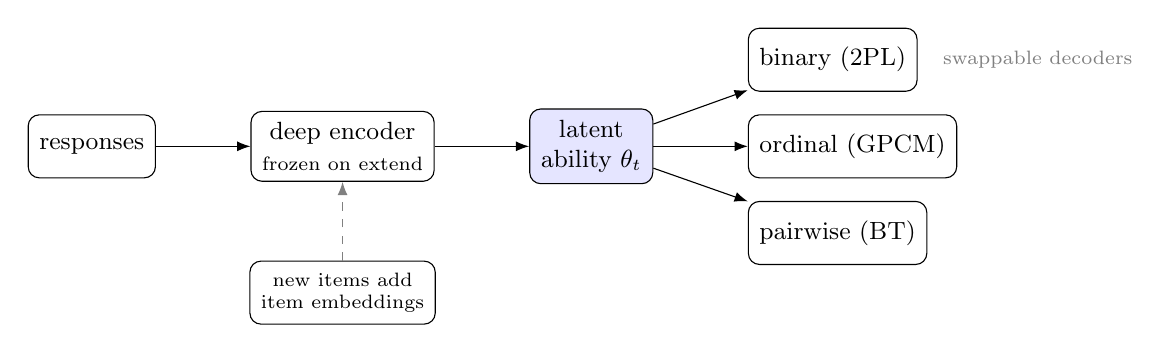
\begin{tikzpicture}[font=\small, node distance=8mm and 12mm,
      box/.style={draw, rounded corners, align=center, minimum height=8mm, inner sep=4pt},
      >=Latex]
    \node[box] (r) {responses};
    \node[box, right=of r] (e) {deep encoder\\{\scriptsize frozen on extend}};
    \node[box, fill=blue!10, right=of e] (t) {latent\\ability $\theta_t$};
    \node[box, right=of t, yshift=11mm] (db) {binary (2PL)};
    \node[box, right=of t] (do) {ordinal (GPCM)};
    \node[box, right=of t, yshift=-11mm] (dp) {pairwise (BT)};
    \draw[->] (r)--(e); \draw[->] (e)--(t);
    \draw[->] (t)--(db); \draw[->] (t)--(do); \draw[->] (t)--(dp);
    \node[box, below=10mm of e, align=center, font=\scriptsize] (ni) {new items add\\item embeddings};
    \draw[->, dashed, gray] (ni) -- (e);
    \node[right=2mm of db, font=\scriptsize, gray] {swappable decoders};
  \end{tikzpicture}}
  \end{center}
  \vspace{0.1em}
  {\small IRT-flavored (interpretable ability, discrimination, step thresholds) and tracking-flavored (dynamic, sequence-based), constrained by neither.}
\end{frame}

\begin{frame}{Three readouts, one scale}
  The encoder maps a response history to a time-varying ability,
  \[ \theta_t = f_\phi(x_{1:t}), \qquad x_t=(\text{item}_t,\ \text{response}_t). \]
  Each decoder is a logistic model of a difference on that one scale, with $\sigma(z)=1/(1+e^{-z})$:
  \begin{align*}
    \text{binary (2PL):}\quad   & P(\text{correct}) = \sigma\!\big(\alpha_j(\theta-\beta_j)\big) \\[2pt]
    \text{ordinal (GPCM):}\quad & P(r{=}k) = \frac{\exp\sum_{c=0}^{k}\alpha_j(\theta-\beta_{j,c})}{\sum_{m=0}^{K-1}\exp\sum_{c=0}^{m}\alpha_j(\theta-\beta_{j,c})} \\[2pt]
    \text{pairwise (BT):}\quad  & P(i \succ j) = \sigma(s_i - s_j)
  \end{align*}
  {\small The pairwise model is Rasch between two items, and Rasch is the binary model between a person and an item. One scale, three readouts.}
\end{frame}

\begin{frame}{How we test it, and how we measure}
  Two evaluation modes, every result labeled as one.
  \begin{itemize}
    \item \textbf{Synthetic recovery.} Responses generated from \emph{known} item parameters and a \emph{known}, moving ability. Check the model recovers them. Exact ground truth.
    \item \textbf{Real transfer on Duolingo SLAM.} Whether item difficulty measured one way predicts it measured another, on real learners.
  \end{itemize}
  \why{We report \textbf{rank recovery} (Spearman) throughout. For item selection and feedback, what matters is whether the model \emph{orders} items and abilities the way the truth does, not whether the numbers match exactly. Rank recovery measures exactly that, and is robust to the skewed difficulty distributions real data shows.}
\end{frame}

\begin{frame}{Result 1. Track ability as it moves}
  \synth\ Each learner's ability follows a random walk, $\theta_{t+1}=\theta_t+\varepsilon_t$, over their answer sequence. The model sees only the responses.
  \begin{center}
    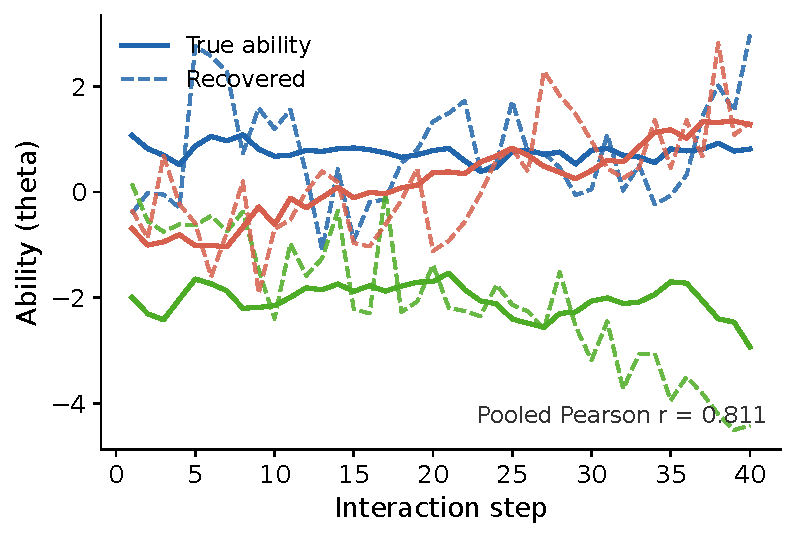
\includegraphics[height=0.5\textheight]{fig_trajectory.pdf}
  \end{center}
  {\small Recovered trajectories follow the true ones. The model infers where ability is heading, not just where it is.}
  \why{Metric: net-drift rank recovery $\rho_s(\hat\Delta,\Delta)$, where $\Delta_p=\theta_{p,T}-\theta_{p,1}$ is each learner's net change. It isolates whether we track the \emph{movement}, separate from the static level.}
\end{frame}

\begin{frame}{How much movement the tracking needs}
  \synth\ Sweeping the size of the drift.
  \begin{center}
    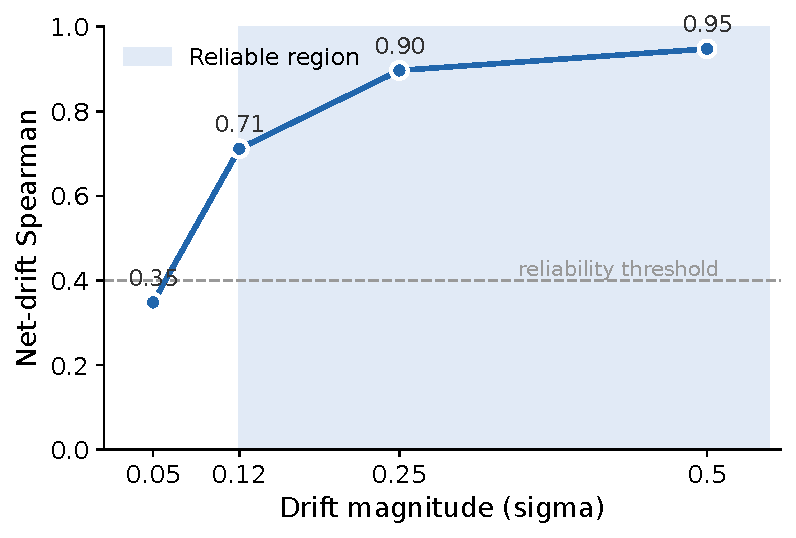
\includegraphics[height=0.5\textheight]{fig_drift_sweep.pdf}
  \end{center}
  {\small Reliable wherever ability meaningfully moves (drift $\geq 0.12$). The gain is precisely in the moving regime, where a static estimate cannot reach.}
  \why{Same net-drift metric as Result 1, swept across how fast ability changes. Low values at near-static are expected, there is barely any change to rank.}
\end{frame}

\begin{frame}{Result 2. One scale across response formats}
  \synth\ One shared item representation, an ordinal (GPCM) head and a pairwise (Bradley-Terry) head, trained jointly. Some items appear \emph{only} in ordinal data, some \emph{only} in pairwise data, the rest in both.
  \begin{center}
    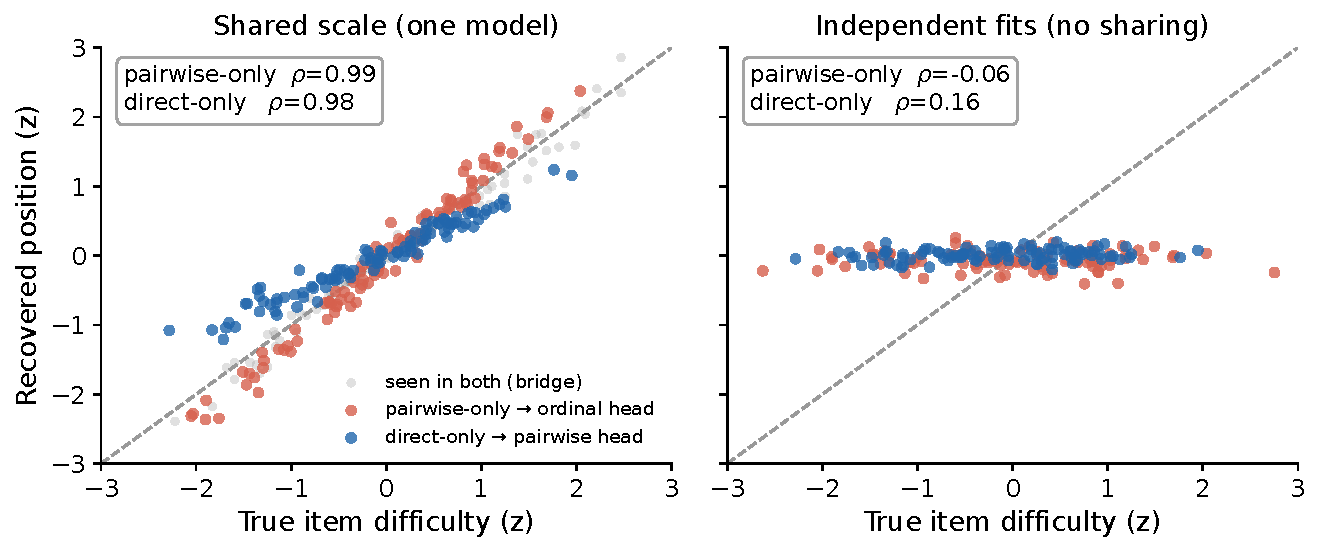
\includegraphics[width=0.93\textwidth]{fig_crossformat.pdf}
  \end{center}
  {\small An item seen only in pairwise comparisons lands on the ordinal scale ($\rho{=}0.99$), and vice versa ($\rho{=}0.98$). Fit the formats independently and the held-out items are noise ($\rho{\approx}0$). The shared representation does the unifying, not a coincidence of ground truth.}
  \why{Metric: Spearman between a held-out-format item's recovered position and its true difficulty. The model never saw these items in the format it is being read out in, so the signal can only arrive through the shared scale, anchored by the items seen in both.}
\end{frame}

\begin{frame}{Result 3. One scale across respondents}
  \real\ A pool of small language models attempt 486 SLAM tap-format items. We grade them and ask whether their item difficulty ranks human item difficulty.
  \begin{center}
    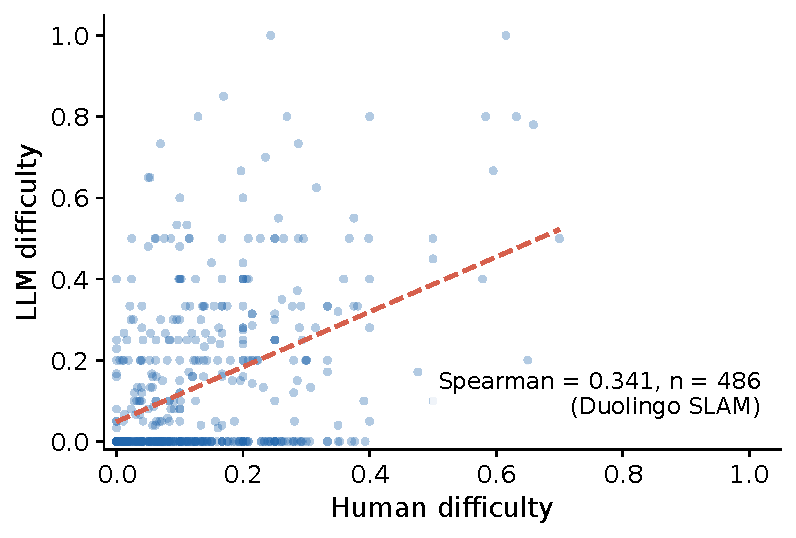
\includegraphics[height=0.46\textheight]{fig_slam_transfer.pdf}
  \end{center}
  {\small Spearman 0.34. A moderate, real signal from a near-homogeneous model pool, so a lower bound a more diverse pool would likely raise.}
  \why{Metric: Spearman between model and human item difficulty (proportion incorrect). Tap-format items are used because there the learner selects from given word tiles, so SLAM's exact-match grading artifact is structurally absent.}
\end{frame}

\begin{frame}{Result 4. Extend the bank cheaply}
  \synth\ New items $E$ attach to the frozen scale by fitting only their own embeddings, the classical fixed-anchor calibration of Kolen and Brennan, reused, not reinvented:
  \[ \min_{\{e_j:\, j\in E\}}\ \sum_{j\in E}\sum_{p} -\log P\big(r_{pj}\mid \theta_p,\, e_j\big), \qquad \phi,\ \{e_j: j\in B\}\ \text{frozen}. \]
  \begin{center}
    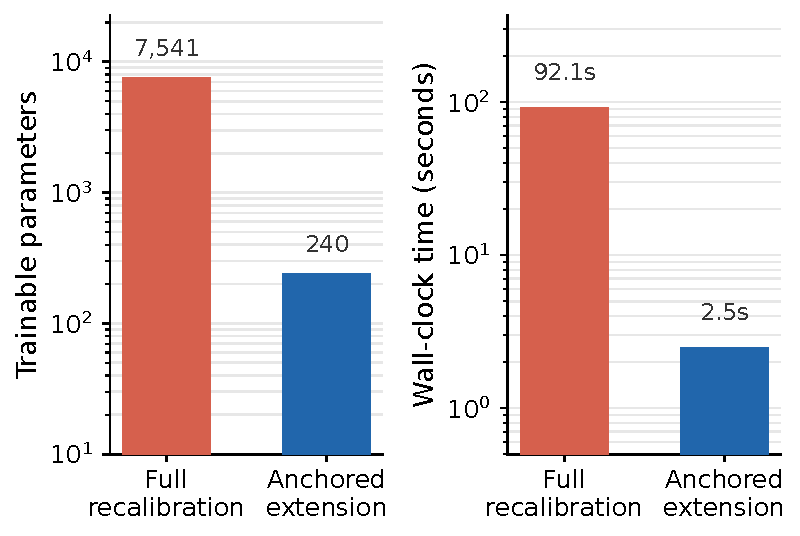
\includegraphics[height=0.4\textheight]{fig_cost.pdf}
  \end{center}
  {\small About 30 times fewer parameters than a full recalibration, and the scale stays stable across repeated rounds with no compounding.}
  \why{The novelty is not the freezing, which is decades old. It is that the frozen scale is a deep encoder that keeps tracking and generalizing. Next slide.}
\end{frame}

\begin{frame}{What is new, against traditional IRT and CAT}
  Fixed-parameter calibration, freezing the scale and anchoring new items, is standard in classical adaptive testing (Kolen and Brennan). We use it. We do not claim it.
  \vspace{0.5em}

  \textbf{What is new is where the scale lives, and what it does.} In classical CAT the scale is a few explicit item parameters, trivial to freeze, and ability is a static estimate on a fixed item pool. Here the scale is a deep encoder, and the frozen encoder
  \begin{itemize}
    \item tracks a \textbf{moving} ability, not a static score,
    \item \textbf{generalizes} to items it never trained on, and
    \item carries \textbf{ordinal and pairwise} responses on one scale, not only right or wrong.
  \end{itemize}
  \vspace{0.3em}
  Classical CAT has no encoder to keep tracking, no moving ability, and no shared format. The freezing is borrowed plumbing. The dynamic, generalizing, format-shared scale is the contribution.
\end{frame}

\begin{frame}{The numbers}
  \centering\small
  \begin{tabular}{llccl}
    \toprule
    Result & Metric & $n$ & Data & Value \\
    \midrule
    Dynamic tracking      & net-drift rank recovery       & 1500 & synthetic       & 0.71--0.95 \\
    Cross-format transfer & held-out item on other scale  & 300  & synthetic       & 0.98--0.99 \\
    Respondent transfer   & model vs human difficulty     & 486  & Duolingo SLAM   & 0.34 \\
    Cheap extension      & params vs full recalibration & ---  & synthetic       & $\sim 30\times$ fewer \\
    Continual extension  & scale drift over 5 rounds   & ---  & synthetic       & none \\
    \bottomrule
  \end{tabular}
  \vspace{0.9em}

  {\footnotesize All correlations are Spearman rank recovery. Synthetic results are a proof of concept; the real-data transfer is moderate and lower-bounded by a near-homogeneous model pool.}
\end{frame}

\begin{frame}{Why this fits a multi-domain platform}
  A platform spanning language, math, music, and chess faces one learner-modeling problem repeated many times.
  \begin{itemize}
    \item One model measures all of them on a single interpretable, extensible scale.
    \item Ordinal grades and longitudinal tracking, the parts a dichotomous line leaves open.
    \item Cheap cold-start for the constant stream of new content.
  \end{itemize}
\end{frame}

\begin{frame}{Status and a concrete next step}
  \textbf{Now.} A single working model, validated as a proof of concept on synthetic data and on a real Duolingo SLAM transfer test, with its reliable operating envelope mapped.
  \vspace{0.6em}

  \textbf{A concrete step together.}
  \begin{itemize}
    \item A slice of partial-credit or ordinal response data, for example graded math or music items, to test the ordinal and longitudinal claims on real learners.
    \item Or a short pilot co-designing a diverse model pool to sharpen the respondent-transfer result.
  \end{itemize}
\end{frame}

\begin{frame}{References}
  \footnotesize
  \begin{itemize}
    \item Kolen and Brennan. Test Equating, Scaling, and Linking. Springer, 2004.
    \item Duolingo SLAM shared task. Second Language Acquisition Modeling, 2018.
    \item AutoIRT. Automated item calibration. Duolingo, 2024.
    \item BanditCAT. Bandit-based adaptive testing for language assessment. Duolingo, 2024.
    \item ma-irt. Deep ordinal item response theory, our groundwork, under review.
  \end{itemize}
\end{frame}

\begin{frame}{Backup. Extension stays stable across rounds}
  \synth\ Five sequential rounds, one hundred new items.
  \begin{center}
    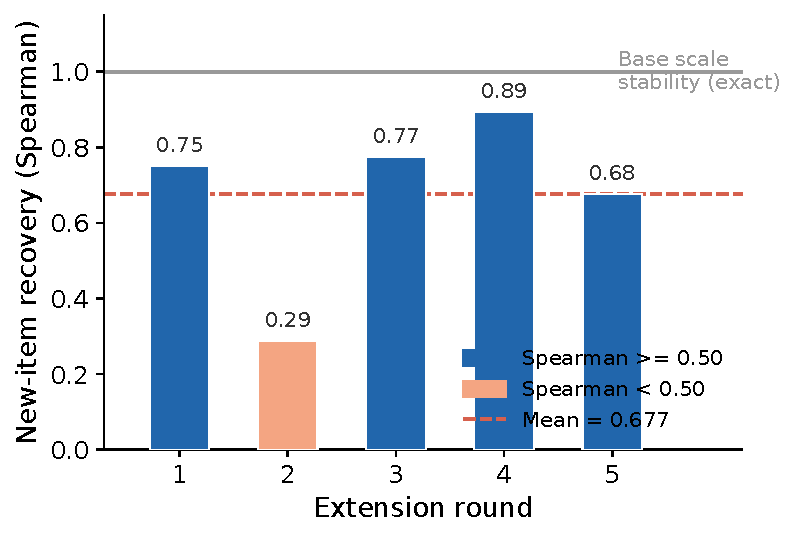
\includegraphics[height=0.52\textheight]{fig_multiround.pdf}
  \end{center}
  {\small The base scale is untouched (stability exact), and per-round new-item recovery stays flat. Error does not compound.}
\end{frame}

\end{document}
